\subsubsection{Envío y recepción de comandos}

Se implementó un sistema de comunicación basado en el protocolo MQTT (Message Queuing Telemetry Transport) para enviar y recibir informacion del robot. Se envían vectores a recorrer con una estructura de datos a modo de tupla de valores que representa la distancia a recorrer, las velocidades lineales y angulares del robot: $distancia [m]$, $V_x [m/seg]$, $V_y [m/seg]$ y $V_\theta [RPM]$.

Además, el robot es capaz de enviar información por medio de MQTT sobre la odometría y el estado en tiempo real. Esto resulta útil dado que posibilita monitorear el estado del robot y realizar ajustes si es necesario.

Por un lado, las velocidades $V_x$ y $V_y$ determinan un sentido de movimiento en linea recta sobre el plano. Por otro lado, $V_\theta$ controla la rotación del robot sobre su propio eje, permitiéndole girar en el plano horizontal.

Cuando se envía una tupla de valores de velocidad mediante MQTT, el robot calcula la velocidad para cada rueda usando el modelo cinemático y establece los motores a la velocidad estipulada, luego se detiene cumplida la distancia recorrida. En la Figura \ref{fig:diagcomponentesp32conmodelocinem} se muestra un diagrama de secuencia con los componentes integrados hasta el momento.

\begin{figure}[H]
    \centering
    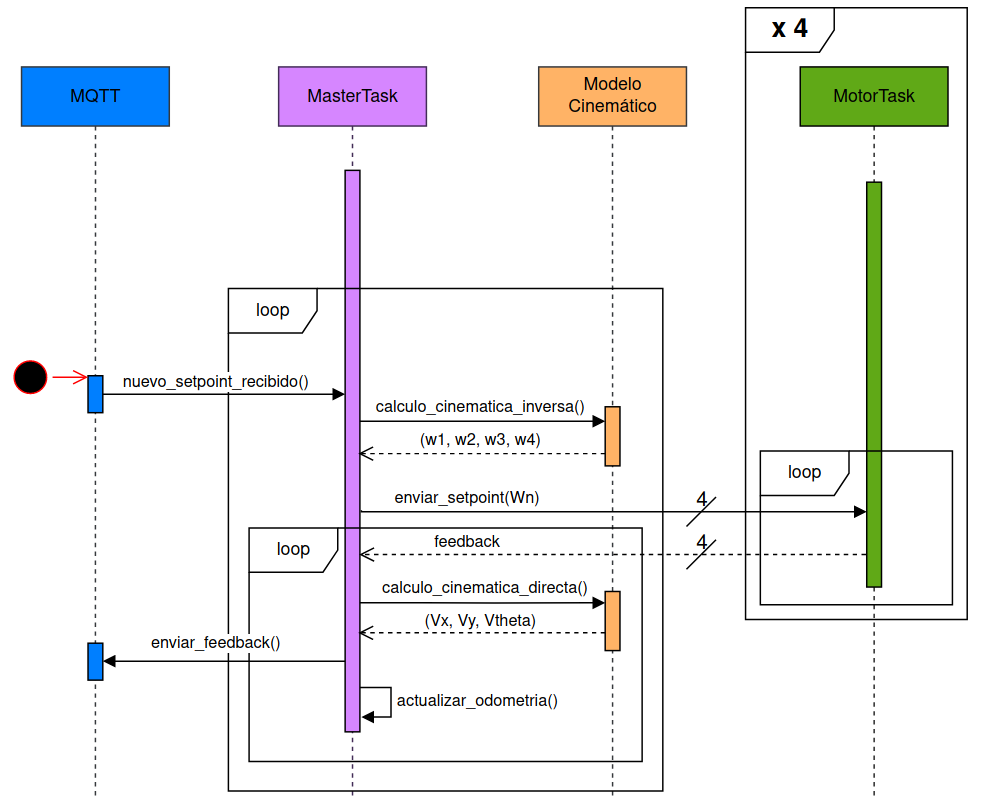
\includegraphics[width=1\linewidth]{images/diag_secuencia_full_modelo_cinematico.png}
    \caption{Diagrama de secuencia de la ESP32 con el Modelo Cinemático}
    \label{fig:diagcomponentesp32conmodelocinem}
\end{figure}
